\documentclass{beamer}

\usetheme[hidefootline,altlogo=images/ssl-logo_text.png,sidebarwidth=1.9cm]{Oxford}
\usepackage{subcaption}

\begin{document}

\title[Spoofing Earth Observation Satellites through Radio Overshadowing]{Firefly: Spoofing Earth Observation Satellites through Radio Overshadowing}
\author[Edd Salkield]{
  \emph{Edd Salkield}
  \inst{1}
  \and
  Joshua Smailes
  \inst{1}
  \and
  Sebastian Köhler
  \inst{1}
  \and
  Simon Birnbach
  \inst{1}
  \and
  Richard Baker
  \inst{1}
  \and
  Martin Strohmeier
  \inst{2}
  \and
  Ivan Martinovic
  \inst{1}
}
\institute[--~~Systems Security Lab]{
  \inst{1} Systems Security Lab, University of Oxford \and %
  \inst{2} Cyber-Defence Campus, armasuisse Science + Technology
}
\date{Trinity Term 2022}

\makeoxfordtitle

\section{Motivation}

\begin{frame}
  \frametitle[Challenges]{Challenges of unauthenticated satellites}
  \begin{itemize}
    \item Many current satellites do not encrypt the downlink, due to:
    \begin{itemize}
      \item Engineering constraints
      \item Desire for public reception
      \item Increased power budget and costs
      \item Legacy systems, and backwards compatibility with them
    \end{itemize}
    \item Other satellites are decryptable, due to:
    \begin{itemize}
      \item Insecure cryptosystems~\footnote{COMS-1 uses single DES \url{https://vksdr.com/lrit-key-dec/}}
      \item Leaked keys~\footnote{GK-2A keys embedded in published source code \url{https://vksdr.com/xrit-rx/}}
    \end{itemize}
  \end{itemize}
\end{frame}

\begin{frame}
  \frametitle{Implications}
  \framesubtitle{Data secrecy}

  \begin{center}
    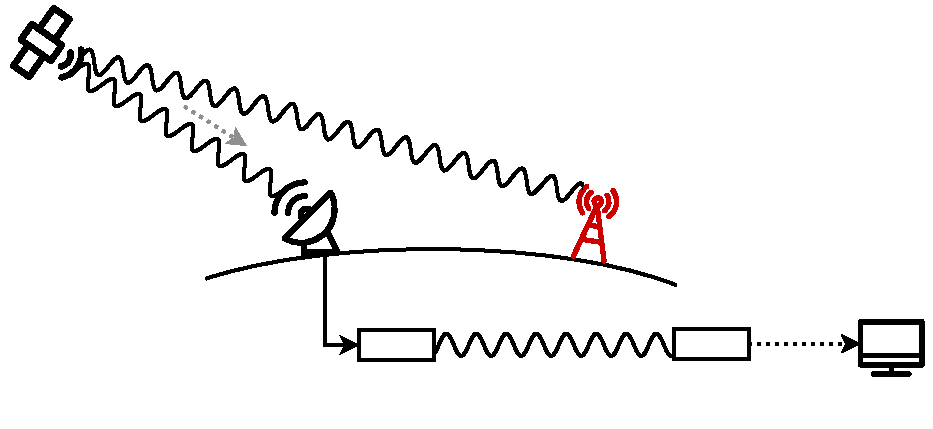
\includegraphics[width=0.7\textwidth]{images/eavesdropping_illustration.pdf}
  \end{center}

  Using only an off-the-shelf SDR and open source software, attackers can:
  \begin{itemize}
    \item Read confidential maritime data and internet traffic, Pavur et. al~\cite{pavur2020tale,pavur2019secrets}
    \item Eavesdrop on Iridium traffic and cals~\cite{iridium-toolkit}
  \end{itemize}

  Certain satellites designed to be unencrypted, e.g.
  \begin{itemize}
    \item EOS fleet: Terra, Aqua, Aura, etc.
    \item Amateur radio satellites e.g. SO-50, QO-100
    \item Freeview TV
  \end{itemize}

  \note{Lack of crypto has resulted in lots of work into eavesdropping}
\end{frame}

\begin{frame}
  \frametitle{Implications}
  \framesubtitle{Data authenticity and integrity}

  \begin{center}
    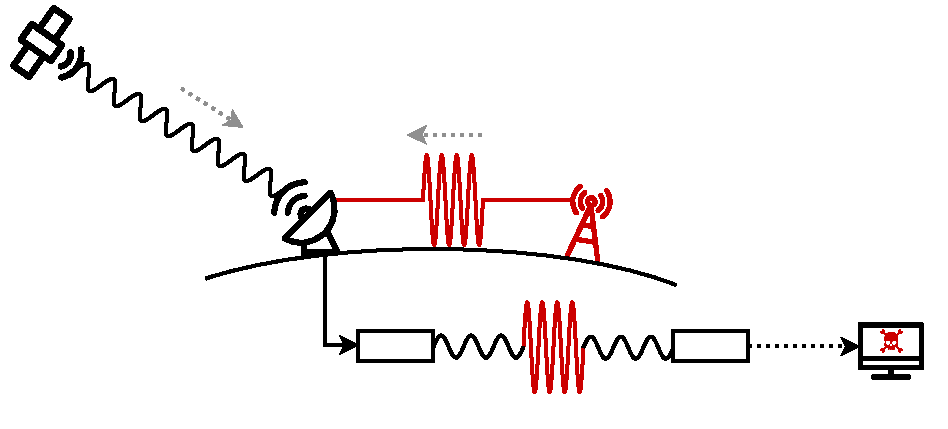
\includegraphics[width=0.7\textwidth]{images/overshadow_illustration.pdf}
  \end{center}

  Spoofing attacks have been shown against:
  
  \begin{itemize}
    \item GNSS to manipulate calculated location~\cite{tippenhauer2011requirements,2204.11641}
    \item Uplink to hijack the satellite or intrude on TV broadcasts~\cite{time_midnight,2011ChinaCongressReport}
  \end{itemize}

  However, no work considers the consequences of spoofing Earth Observation satellites.

  Research question: What can the attacker achieve by exploiting the unauthenticated channel?
  \note{No work considers overshadowing in a more general case}
\end{frame}

\begin{frame}
  \frametitle{Implications}
  \framesubtitle{Unencrypted Earth Observation Satellites}

  Many Earth Observation satellites are unencrypted, including:

  \begin{itemize}
    \item \textbf{Fire detection and management} e.g. Terra, Aqua
    \item Geospatial intelligence e.g. Landsat-7..9
    \item Weather monitoring e.g. GOES-14..17, NOAA=15,18..21, FengYun series
    \item Infrared sensing e.g. Metop-A,B
    \item Climate monitoring e.g. Suomi-NPP
  \end{itemize}
\end{frame}

\subsection{Threat model}
\begin{frame}
  \frametitle{Threat model}
  \framesubtitle{Adversary's goal}

  \begin{center}
    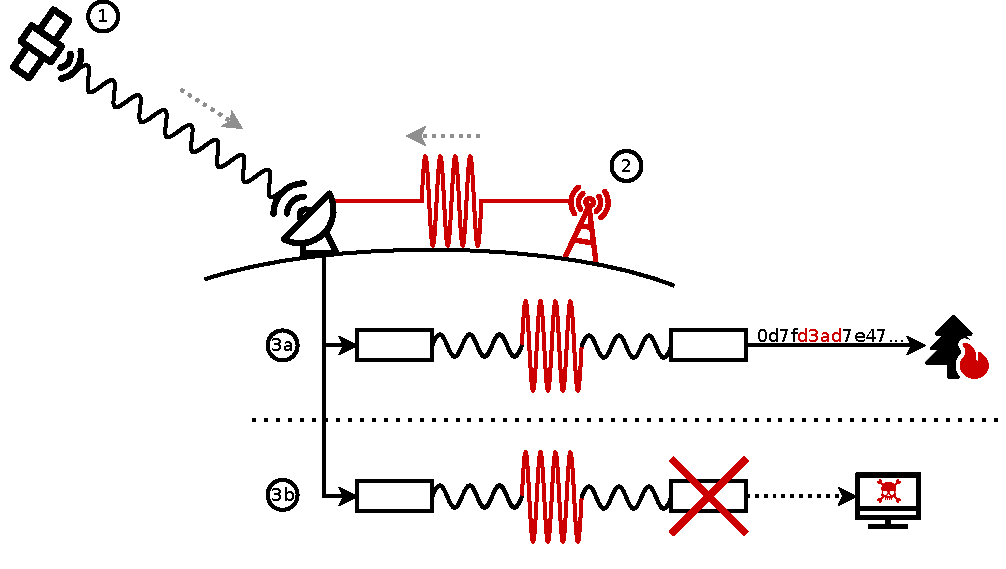
\includegraphics[width=0.7\textwidth]{images/attack_illustration.pdf}
  \end{center}

  Attacker transmits counterfeit signals in the vicinity of the receiver, to:
  \newline
  \begin{itemize}
    \item Affect the satellite-derived datasets
    \item Exploit or disrupt downlink processing stages
  \end{itemize}

  \note{
      \begin{itemize}
        \item Inject false data, disrupting automated detection systems.
        \item Mask real data, denying people information.
      \end{itemize}

      \begin{itemize}
        \item Achieve denial of service, e.g. by causing pipeline stages to crash.
        \item Execute arbitrary code, e.g. by exploiting processing stages that call the shell.
      \end{itemize}
  }
\end{frame}

\subsection{Attacker capabilities}

\begin{frame}
  \frametitle{Attacker capabilities}
  \framesubtitle{Estimated cost}
  \centering
  \begin{tabular}{ l | l }
    \textbf{Hardware component} & \textbf{Cost} \\
    \hline
    limeSDR & $598$ USD \\
    X-Band transmitter & $22,800$ EUR \\
    Compatible antenna & $6,400$ EUR \\
    \hline
    Total & \~{}$30,000$ EUR
  \end{tabular}

  Within the budget of a motivated hobbyist.
\end{frame}

\section{Case Study: FIRMS}
\subsection{Experiment setup}

\begin{frame}
  \frametitle{Case Study: Forest fire detection in FIRMS}
  \framesubtitle{NASA's global fire detection service}
  \centering
  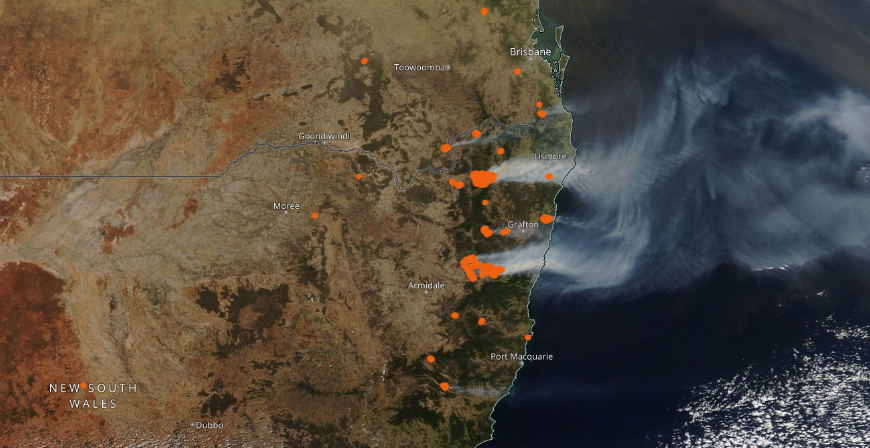
\includegraphics[width=\columnwidth]{images/bushfire.png}
  \newline
  The 2019 Australia bushfires as seen from Aqua's MODIS instrument, annotated with the \textit{Fires and Thermal Anomalies} dataset on NASA's worldview.
\end{frame}

\begin{frame}
  \frametitle{Case Study: Forest fire detection in FIRMS}
  \framesubtitle{Experiment setup}

  \begin{center}
    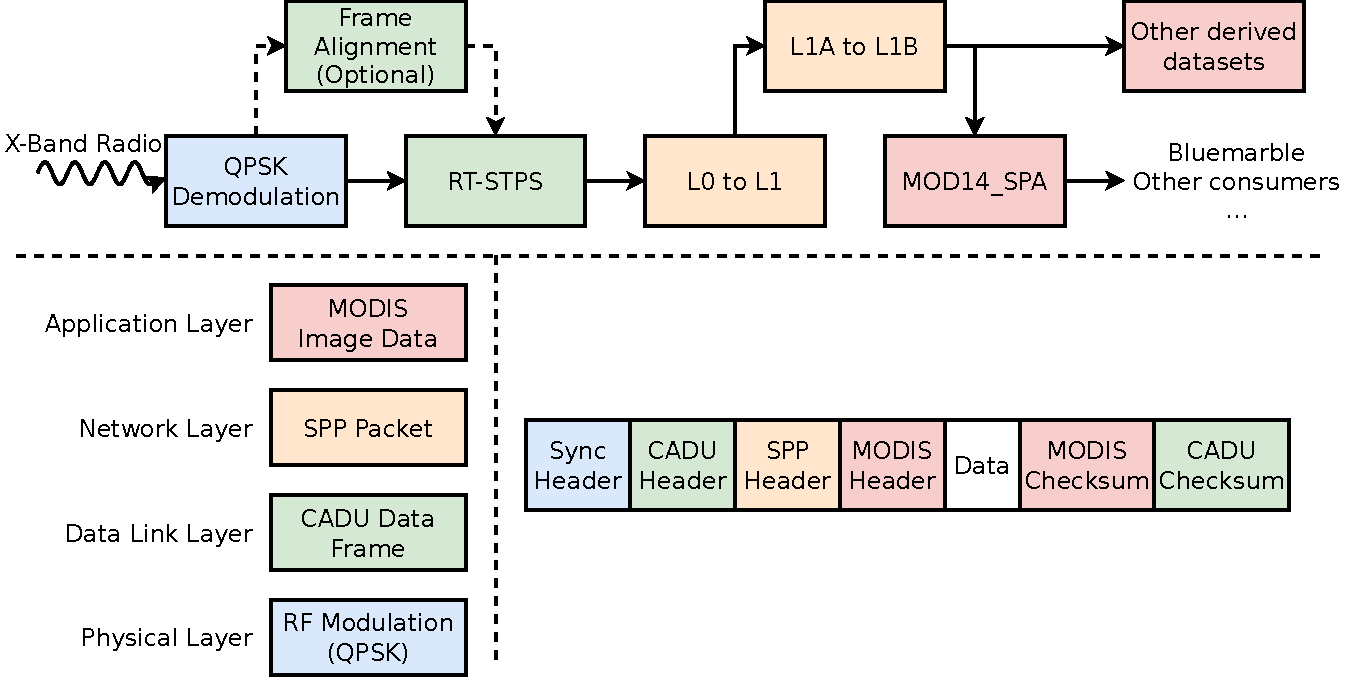
\includegraphics[width=0.8\textwidth]{images/attack_types.pdf}
  \end{center}

  We set up docker pipeline for the relevant parts of IPOPP
\end{frame}

\begin{frame}
  \frametitle{Exploiting processing stages}
  \framesubtitle{Obtaining the processing software}
  \centering
  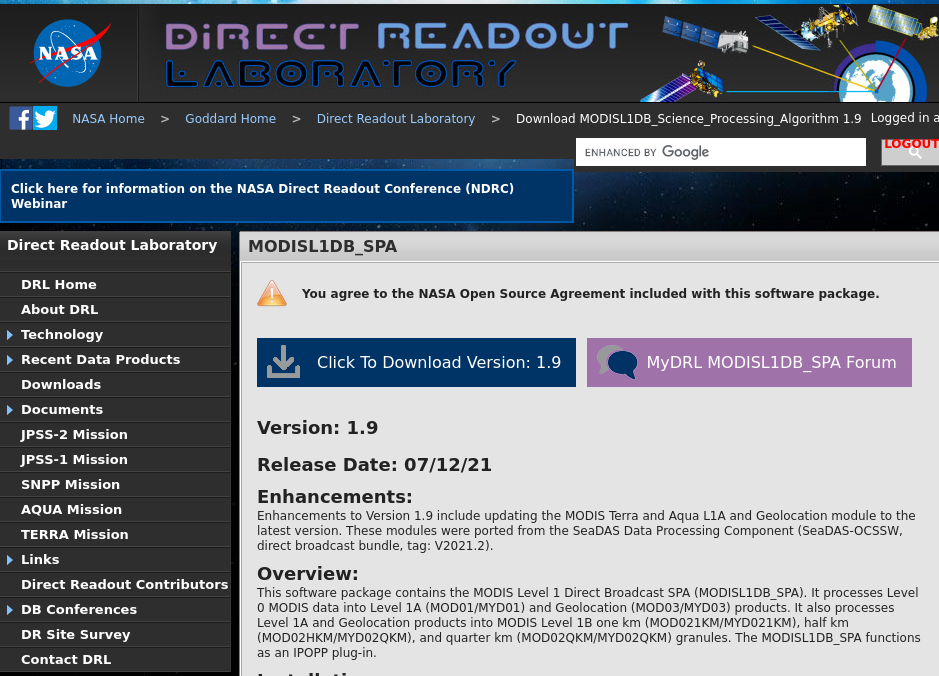
\includegraphics[width=0.7\textwidth]{images/drl.png}
  \newline
  With a research account, anyone can download the entire set of decoding software from NASA's \textit{Direct Readout Laboratory}
  \newline
  \url{https://directreadout.sci.gsfc.nasa.gov/}
\end{frame}

\subsection{Affecting the derived dataset}

\begin{frame}
  \frametitle{Affecting the derived dataset}
  \framesubtitle{Key challenges}
  \begin{itemize}
    \item Obtaining legitimate data
    \begin{itemize}
      \item Beforehand -- download from NASA distributed data archive
      \item Live -- set up custom receiver setup
    \end{itemize}

    \item Processing it to add/remove artefacts
    \begin{itemize}
      \item Reverse engineer the image format, and write an image manipulation program
    \end{itemize}
  \end{itemize}
\end{frame}

\begin{frame}
  \frametitle{Affecting the derived dataset}
  \framesubtitle{Data capture}
  \centering
  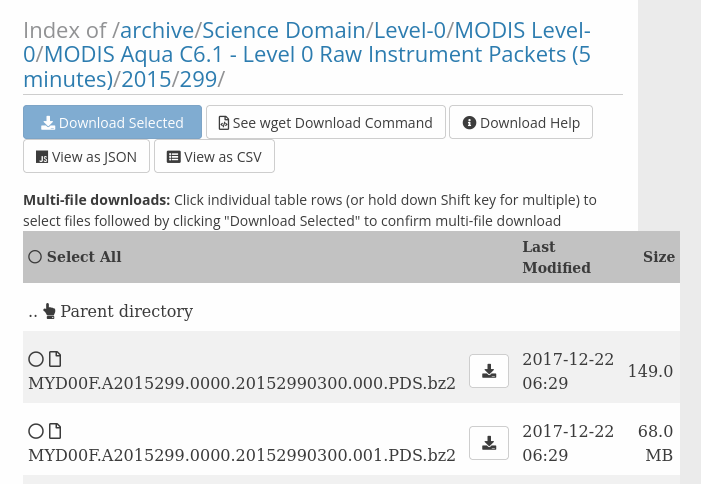
\includegraphics[width=0.8\textwidth]{images/level0.png}
  \url{https://ladsweb.modaps.eosdis.nasa.gov/archive/}
\end{frame}

\begin{frame}
  \frametitle{Affecting the derived dataset}
  \framesubtitle{Data processing: image format reversing}
  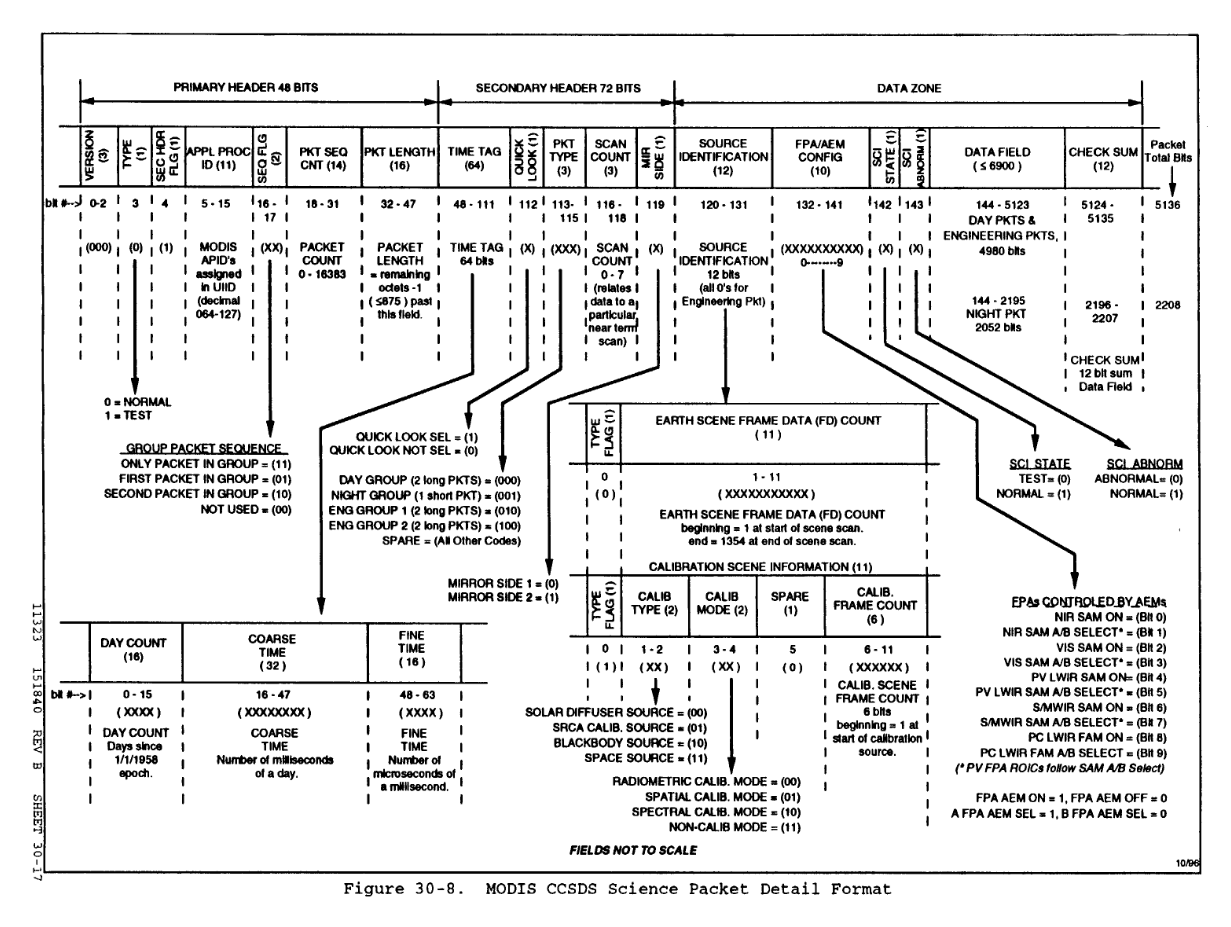
\includegraphics[width=\textwidth]{images/image_format.png}
  \note{It's not as easy as drawing dots on}
\end{frame}

\begin{frame}
  \frametitle{Affecting the derived dataset}
  \framesubtitle{Data processing: building protocol manipulation tools}

  \textbf{TODO: find way of presenting the tools}
\end{frame}

\begin{frame}
  \frametitle{Attack consequences}
  \framesubtitle{Affecting the derived dataset}
  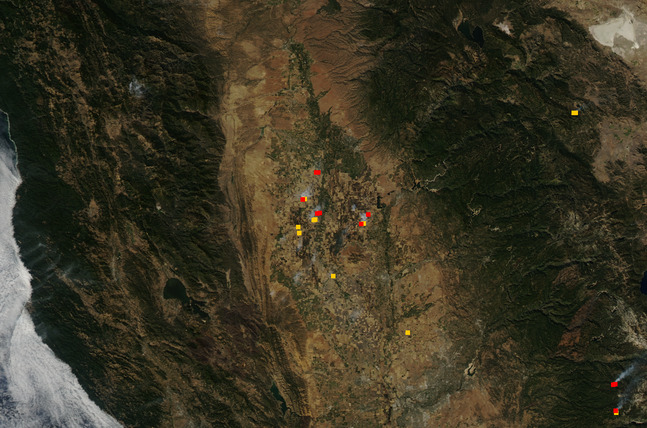
\includegraphics[width=\textwidth]{images/injection/original.jpg}
  \newline
  \centering
  Original image.
\end{frame}

\begin{frame}
  \frametitle{Attack consequences}
  \framesubtitle{Affecting the derived dataset}
  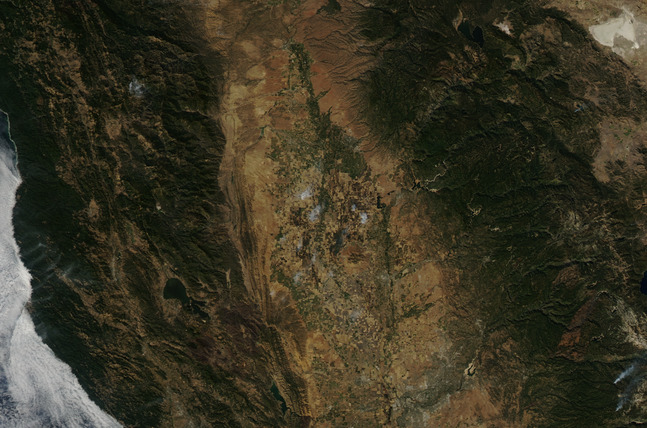
\includegraphics[width=\textwidth]{images/injection/masked_0.jpg}
  \newline
  \centering
  Masking existing fires.
\end{frame}

\begin{frame}
  \frametitle{Attack consequences}
  \framesubtitle{Affecting the derived dataset}
  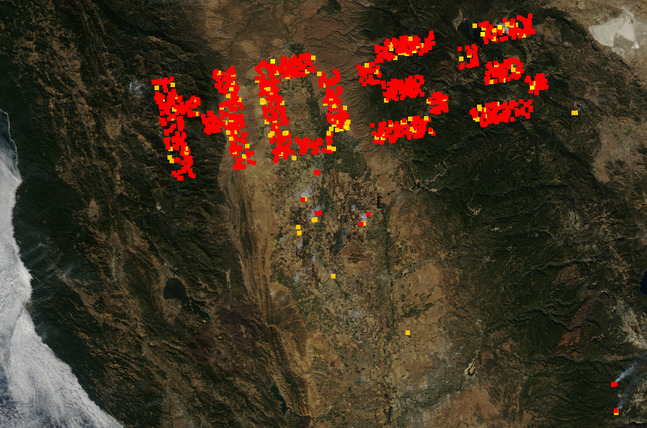
\includegraphics[width=\textwidth]{images/injection/pixels_800_140.jpg}
  \newline
  \centering
  Fine-grained control over fire injection.
\end{frame}

\subsection{Exploiting processing stages}

\begin{frame}
  \frametitle{Exploiting processing stages}
  \framesubtitle{Key challenges}
  \begin{itemize}
   \item Obtain downlink decoder software and perform security audit
   \begin{itemize}
     \item Look for possible exploits around manual memory management and execution boundaries
   \end{itemize}
    \item Construct payload packet to trigger vulnerability chain
    \begin{itemize}
      \item Violate assumptions about the protocol headers
    \end{itemize}
  \end{itemize}
\end{frame}


\begin{frame}
  \frametitle{Exploiting processing stages}
  \framesubtitle{Construct payload packet}
  \centering
  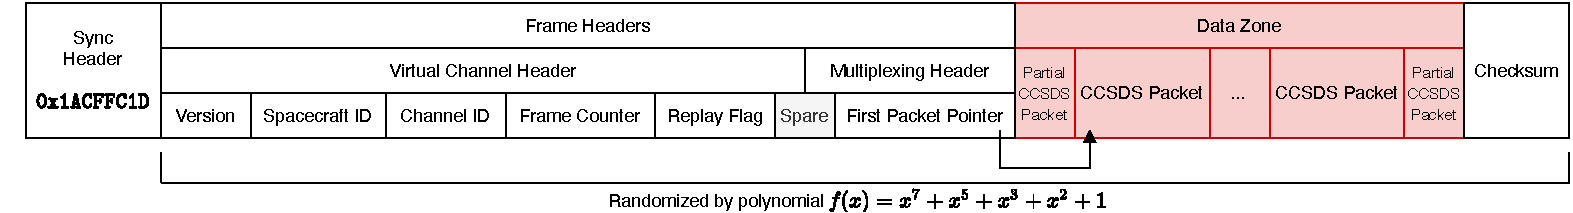
\includegraphics[width=\textwidth]{images/cadu_diagram.pdf}
  \note{Number of causes of concern: L0 to L1 made of many disparate components, interacting across boundaries with access to the shell. Using C programs that don't pay huge attention to managing memory correctly, and using a slightly buggy protocol header parser.}
\end{frame}


\begin{frame}
  \frametitle{Attack consequences}
  \framesubtitle{Exploiting the processing stages}
  \centering
  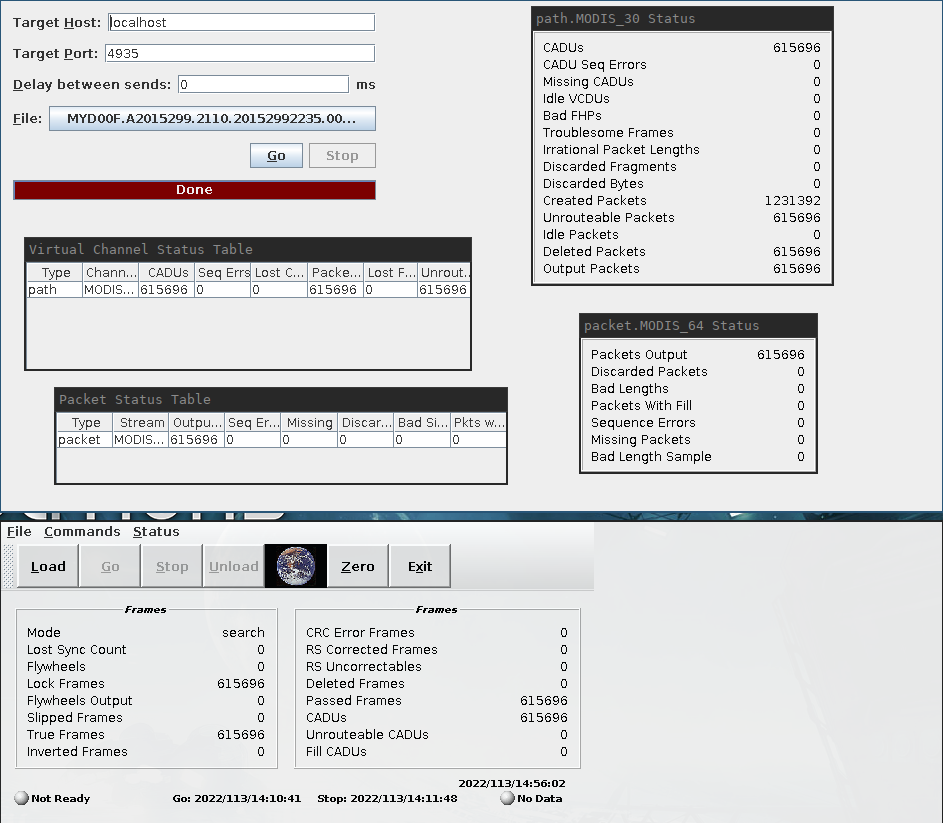
\includegraphics[width=0.7\textwidth]{images/rtstps_correct.png}
\end{frame}

\begin{frame}
  \frametitle{Attack consequences}
  \framesubtitle{Exploiting the processing stages}
  \centering
  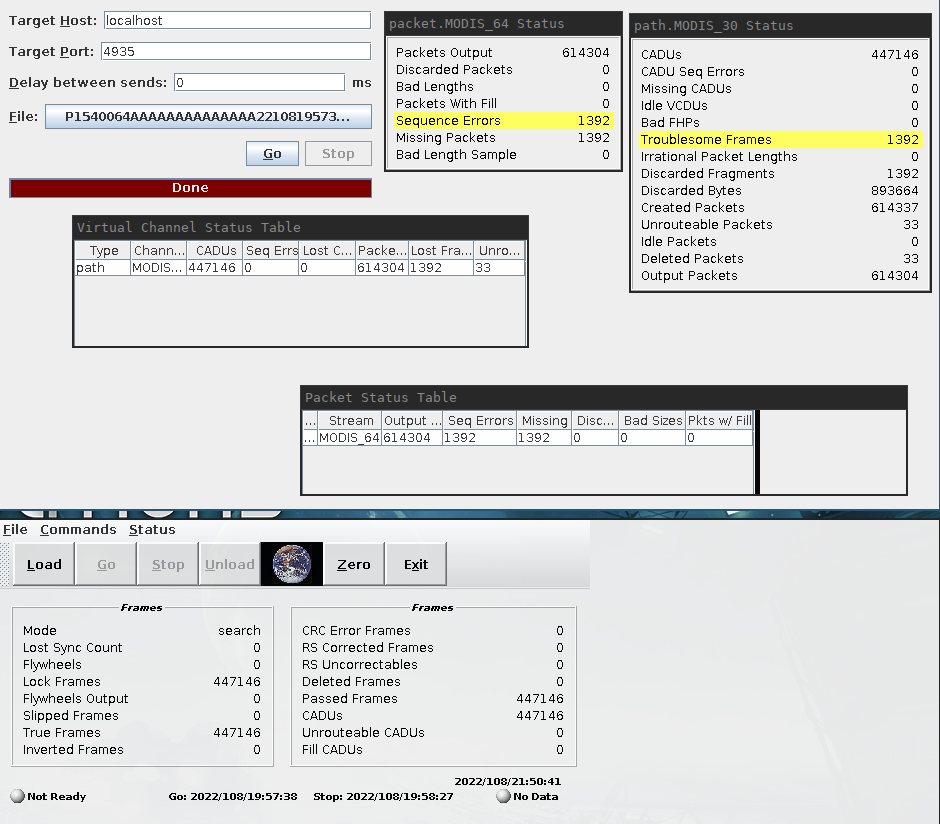
\includegraphics[width=0.7\textwidth]{images/rtstps_incorrect.png}
\end{frame}

\section{Countermeasures}
\note{Cryptography is infeasible because of reasons discussed earlier}
\subsection{Multi-receiver data comparison}
\begin{frame}
  \frametitle{Countermeasures}
  \framesubtitle{Multi-receiver data comparison}
  \textbf{TODO: citations}
  Look for artefacts of tampering in the packets, and compare packets from multiple groundstations

  \begin{itemize}
    \item Certain systems already have multiple receiver stations
    \item Protects against decoder exploitation
    \item Doesn't require any hardware modifications to the receiver
  \end{itemize}
\end{frame}

\subsection{Timing analysis}
\begin{frame}
  \frametitle{Countermeasures}
  \framesubtitle{Timing analysis}

  \begin{itemize}
    \item Triangulating the source effective in other systems such as aircraft
    \item Calculated position can be compared against orbital parameters
    \item Requires accurate clock synchronisation and multiple receivers
  \end{itemize}
\end{frame}

\subsection{Physical-layer fingerprinting}
\begin{frame}
  \frametitle{Countermeasures}
  \framesubtitle{Physical-layer fingerprinting}

  \begin{itemize}
    \item Analyse properties of the legitimate/overshadowed signal
    \item Only effective on the downlink
    \item Traditional approaches like analysing signal-to-noise may prove effective
    \item New ML approaches starting to be created (PAST-AI)
  \end{itemize}
\end{frame}

\section{Conclusion}

\begin{frame}
  \frametitle{Conclusion}

  Our paper...
  \begin{itemize}
    \item presents a demonstration of byte-level spoofing against NASA's forest fire detection system.
    \item provides the source code required to manipulate the packet data and structure.
    \item confirms that only a moderate budget is required to perform these attacks.
    \item identifies current countermeasures which significantly increase attack difficulty.
  \end{itemize}
\end{frame}

% TODO: end card with socials, contact details, etc.
\end{document}
